\chapter{FormL3SS:\,\\Protecting User Secrets on the Client}
\label{chp::formless}

In Chapter \ref{chp3::breaches}, we found that Man-in-the-Browser (MitB) malware (also known as \textit{form grabbers}, \textit{skimmers}, or \textit{magecart-style attacks}) can silently exfiltrate sensitive user data from web forms. As users interact increasingly with browsers and websites, the risk of sensitive data such as passwords and credit card details being stolen by MitB malware and form grabbers increases. These threats can cause serious financial and information loss. To counter such risks, we propose an alternative security measure: an out-of-band mobile phone system that protects against compromised browsers and malicious form manipulation. This chapter presents our system \formless, which includes a standardised protocol for secure information requests and integrates blockchain technology for identity verification. We showcase the effectiveness of the proposed system in securely transmitting data to a trusted server, demonstrating a fusion of traditional security techniques with blockchain systems.

\section{Introduction}
Form grabbers and Man-in-the-Browser (MitB) malware attacks are an effective method of stealing sensitive information and web traffic data. They can be used to steal credit card details, personal information and passwords, which are then auctioned off~\cite{dupont_darkode:_2017} or directly used for fraud and the financial benefit of the attacker. Once the user's machine is infected, there is little modern browsers can do. The Trojans and form grabbers act silently as the user interacts with the web page. One method of circumventing compromised browsers and operating systems is by using another device to submit the data (an out-of-band system).

In this chapter, we are concerned with a secure method of submitting data (typically done via a web form) by the user to the web server (which is hosting the website). We present a design, called \formless, and a proof-of-concept implementation of an out-of-band form submission technique that can securely transfer required data (e.g., payment information) to the trusted server hosting the web application. We design and implement the proposed system on top of a blockchain-based identification and authentication system, \deeid. \deeid already offers passwordless and out-of-band authentication. Moreover, \deeid offers the ability to send messages to the user via a secure communication channel.

Form grabbers and MitB attacks are channelled through various methods. Here, we focus on two: Trojans and malicious third-party JavaScripts injected into the page.

MitB Trojans or financial malware silently infect a device and monitor outgoing communication before it is encrypted. Targeted Trojans attack online banking and ecommerce websites. ZeuS and SpyEye are two famous examples of such Trojans. Recent examples such as BackSwap \cite{kessem_backswap_2018} tailor their code to target specific banks, in this case Spanish banks.

Trojans are inherently form grabbers, but in this context we will refer to form grabbers to scripts that infect third-party libraries. It is common for most web applications to use third-party libraries, mostly JavaScript, to enhance the functionality of the web page. Compromised libraries once loaded into a web page can scrape forms and steal information as they are entered into HTML forms. The most prominent example of such form-grabbing attack is the British Airways (BA) 2018 breach \cite{noauthor_how_nodate} where \num{380000} customer payment details (including CVV numbers) were stolen as they were typed into the page between Aug 21 and Sep 5. The attackers did not compromise the BA's servers, but managed to compromise a third party library called \texttt{modernizr.js}. The attackers injected 22 lines of JavaScript code \cite{j_schwartz_riskiq_nodate} (as shown in Listing \ref{lst::forml3ss::ba-hack}) that sent form data as they were submitted to a rogue phishing server.
\begin{listing}[t]
\begin{minted}
[
frame=lines,
framesep=2mm,
baselinestretch=0.9,
fontsize=\footnotesize,
]
{javascript}
window.onload = function() {
    jQuery("#submitButton").bind("mouseup touchend", function(a) {
        var n = {};
        jQuery("#paymentForm").serializeArray().map(function(a) {
            n[a.name] = a.value
        });
        var e = document.getElementById("personPaying").innerHTML;
        n.person = e;
        var t = JSON.stringify(n);
        
        setTimeout(function() {
            jQuery.ajax({
                type: "POST",
                async: !0,
                url: "https://baways.com/gateway/app/dataprocessing/api/",
                data: t,
                datatype: "application/json"
            })
        }, 500)
    })
};
\end{minted}
\caption{Javascript code that was injected into the British Airways website.}
\label{lst::forml3ss::ba-hack}
\end{listing}
The financial and economic cost of these attacks should be taken seriously. Not only do victims face financial losses, but services providers such as British Airways (BA) can also be fined for putting their customers in danger. BA faces a £183 million fine by the UK regulators (ICO) \cite{noauthor_british_2019}.

With an increasing number of individuals using the Internet for online banking, shopping, etc. The pool of potential victims is only increasing in size. The importance of protecting users whilst enhancing their experience is evident, and thus we shall propose a method to circumvent MitB type attacks and allow the user to transact securely even if the browser or the operating system is untrustworthy compromised.

\section{Design}
\label{sec::forml3ss::design}

The goal of the proposed system, \formless, is to circumvent compromised operating systems, browsers and malicious third party JavaScript libraries (form grabbers), thus creating a secure link between the user and the trusted server (the server hosting the website that the user is interacting with) in order to send sensitive data (e.g. payment information). We are countering two types of attacks: 1) Man-in-the-Browser Trojans such as \textit{ZeuS} and \textit{SpyEye} (also known as financial malware). 2) Form grabbers: Malicious third party libraries that scrape the web page and send the data to a controlled server. Malicious browser extensions fall between those two forms of attack. Therefore, we assume that all interactions and data on the web page displayed on the infected client can be manipulated and altered. The proposed system, \formless, is shown in Figure~\ref{fig:thesys}. The communication flow between the different components of \formless is show in Figure~\ref{fig::forml3ss-sequence}.

\begin{figure}[ht]
\centering
\begin{tikzpicture}[
    >=Stealth,
    actor/.style={rectangle, draw, minimum width=2cm, minimum height=0.4cm},
    message/.style={->, thick},
    return/.style={->, dashed},
    note/.style={rectangle, draw, dashed, fill=yellow!20, align=left, font=\footnotesize}
]

\node[actor] (browser) at (0,0) {Browser};
\node[actor] (server) at (4,0) {Server};
\node[actor] (mobile) at (8,0) {Mobile App};
\node[actor] (chain) at (12,0) {Blockchain};

\draw[dashed] (browser) -- ++(0,-16);
\draw[dashed] (server) -- ++(0,-16);
\draw[dashed] (mobile) -- ++(0,-16);
\draw[dashed] (chain) -- ++(0,-16);

\node[above=0.3cm of browser] {\textbf{Initial Registration}};

\draw[message] (0,-1) -- (4,-1) node[midway, above, font=\scriptsize] {1. Request form};
\draw[message] (4,-2) -- (0,-2) node[midway, above, font=\scriptsize] {2. Signed QR data};
\draw[message] (0,-3) -- (8,-3) node[midway, above, font=\scriptsize] {3. User scans QR};
\node[note, right] at (8,-4) {User manually\\enters domain};
\draw[message] (8,-5) -- (12,-5) node[midway, above, font=\scriptsize] {4. Verify signature};
\draw[return] (12,-5.5) -- (8,-5.5) node[midway, above, font=\scriptsize] {Public key};
\node[note, right] at (8,-6.5) {Store trusted\\relationship};
\draw[message] (8,-7.5) -- (4,-7.5) node[midway, above, font=\scriptsize] {5. Submit data (HTTPS)};
\draw[message] (4,-8) -- (0,-8) node[midway, above, font=\scriptsize] {6. Confirm (WebSocket)};

% Second scenario: In this scenario, the user doesn't have to input domain again (nice)
\node[above] at (6,-10) {\textbf{Subsequent Form Submission}};

\draw[message] (0,-11) -- (4,-11) node[midway, above, font=\scriptsize] {1. Request form};
\draw[message] (4,-12) -- (0,-12) node[midway, above, font=\scriptsize] {2. Signed QR data};
\draw[message] (0,-13) -- (8,-13) node[midway, above, font=\scriptsize] {3. User scans QR};
\node[note, right] at (8,-14) {\textcolor{green!50!black}{Auto-verify}\\No manual input};
\draw[message] (8,-15) -- (4,-15) node[midway, above, font=\scriptsize] {4. Submit data (HTTPS)};
\draw[message] (4,-15.5) -- (0,-15.5) node[midway, above, font=\scriptsize] {5. Confirm (WebSocket)};

\end{tikzpicture}
\caption{\formless communication flow. Here we see how the different components interact with each other and the two scenarios if the user has interacted with the service before.}
\label{fig::forml3ss-sequence}
\end{figure}

\begin{figure}
    \centering
    \textbf{\formless: Design of the Proposed System}
    \linebreak
\tikzset{every picture/.style={line width=0.75pt}} %set default line width to 0.75pt    
\begin{tikzpicture}[x=0.75pt,y=0.75pt,yscale=-0.8,xscale=0.8]
%uncomment if require: \path (0,471); %set diagram left start at 0, and has height of 471

%Rounded Rect [id:dp9341566578511238] 
\draw  [color={rgb, 255:red, 255; green, 255; blue, 255 }  ,draw opacity=1 ][fill={rgb, 255:red, 126; green, 211; blue, 33 }  ,fill opacity=1 ] (259,375.08) .. controls (259,372.28) and (261.28,370) .. (264.08,370) -- (297.02,370) .. controls (299.82,370) and (302.1,372.28) .. (302.1,375.08) -- (302.1,439.92) .. controls (302.1,442.72) and (299.82,445) .. (297.02,445) -- (264.08,445) .. controls (261.28,445) and (259,442.72) .. (259,439.92) -- cycle ;
%Shape: Rectangle [id:dp09480108363402917] 
\draw  [color={rgb, 255:red, 0; green, 0; blue, 0 }  ,draw opacity=0 ][fill={rgb, 255:red, 155; green, 155; blue, 155 }  ,fill opacity=1 ] (116,42.2) -- (431.5,42.2) -- (431.5,333.2) -- (116,333.2) -- cycle ;
%Shape: Rectangle [id:dp7021329026819214] 
\draw  [color={rgb, 255:red, 0; green, 0; blue, 0 }  ,draw opacity=0 ][fill={rgb, 255:red, 255; green, 255; blue, 255 }  ,fill opacity=1 ] (129,114) -- (418.5,114) -- (418.5,319) -- (129,319) -- cycle ;
%Rounded Single Corner Rect [id:dp44180586388155163] 
\draw  [color={rgb, 255:red, 0; green, 0; blue, 0 }  ,draw opacity=0 ][fill={rgb, 255:red, 255; green, 255; blue, 255 }  ,fill opacity=1 ] (302.5,90.4) .. controls (302.5,85.76) and (298.74,82) .. (294.1,82) -- (137,82) -- (137,114) -- (302.5,114) -- cycle ;
%Flowchart: Connector [id:dp652624003566018] 
\draw  [color={rgb, 255:red, 83; green, 48; blue, 48 }  ,draw opacity=0 ][fill={rgb, 255:red, 208; green, 2; blue, 27 }  ,fill opacity=1 ] (127,62) .. controls (127,57.03) and (131.03,53) .. (136,53) .. controls (140.97,53) and (145,57.03) .. (145,62) .. controls (145,66.97) and (140.97,71) .. (136,71) .. controls (131.03,71) and (127,66.97) .. (127,62) -- cycle ;
%Flowchart: Connector [id:dp650021508003567] 
\draw  [color={rgb, 255:red, 83; green, 48; blue, 48 }  ,draw opacity=0 ][fill={rgb, 255:red, 253; green, 255; blue, 15 }  ,fill opacity=1 ] (150,62) .. controls (150,57.03) and (154.03,53) .. (159,53) .. controls (163.97,53) and (168,57.03) .. (168,62) .. controls (168,66.97) and (163.97,71) .. (159,71) .. controls (154.03,71) and (150,66.97) .. (150,62) -- cycle ;
%Flowchart: Connector [id:dp41576241972786043] 
\draw  [color={rgb, 255:red, 83; green, 48; blue, 48 }  ,draw opacity=0 ][fill={rgb, 255:red, 126; green, 211; blue, 33 }  ,fill opacity=1 ] (172,62) .. controls (172,57.03) and (176.03,53) .. (181,53) .. controls (185.97,53) and (190,57.03) .. (190,62) .. controls (190,66.97) and (185.97,71) .. (181,71) .. controls (176.03,71) and (172,66.97) .. (172,62) -- cycle ;
%Shape: Rectangle [id:dp8838213329500311] 
\draw  [color={rgb, 255:red, 1; green, 163; blue, 5 }  ,draw opacity=1 ][fill={rgb, 255:red, 126; green, 211; blue, 33 }  ,fill opacity=1 ] (216.3,195) -- (340.3,195) -- (340.3,315.2) -- (216.3,315.2) -- cycle ;
%Image [id:dp01872814299643899] 
\draw (277.75,254.75) node  {
\includegraphics[width=37pt,height=37pt]{figs/forml3ss/qr.png}};
%Image [id:dp19372135706713323] 
\draw (412,114) node  {
\includegraphics[width=52.5pt,height=52.5pt]{figs/forml3ss/devil.png}};
%Shape: Cube [id:dp5743416341148022] 
\draw  [color={rgb, 255:red, 65; green, 117; blue, 5 }  ,draw opacity=1 ][fill={rgb, 255:red, 255; green, 255; blue, 255 }  ,fill opacity=1 ] (505,157) -- (523,139) -- (565,139) -- (565,219) -- (547,237) -- (505,237) -- cycle ; \draw  [color={rgb, 255:red, 65; green, 117; blue, 5 }  ,draw opacity=1 ] (565,139) -- (547,157) -- (505,157) ; \draw  [color={rgb, 255:red, 65; green, 117; blue, 5 }  ,draw opacity=1 ] (547,157) -- (547,237) ;
%Straight Lines [id:da7598573925900223] 
\draw [color={rgb, 255:red, 65; green, 117; blue, 5 }  ,draw opacity=1 ]   (516.67,189.33) -- (537.67,189.13) ;


%Shape: Rectangle [id:dp15486918257454896] 
\draw  [color={rgb, 255:red, 65; green, 117; blue, 5 }  ,draw opacity=1 ] (512.83,170) -- (541.5,170) -- (541.5,175.5) -- (512.83,175.5) -- cycle ;
%Shape: Rectangle [id:dp34848405551077777] 
\draw  [color={rgb, 255:red, 65; green, 117; blue, 5 }  ,draw opacity=1 ] (512.83,179.33) -- (541.5,179.33) -- (541.5,184.83) -- (512.83,184.83) -- cycle ;
%Shape: Rectangle [id:dp5102034164356797] 
\draw  [color={rgb, 255:red, 255; green, 255; blue, 255 }  ,draw opacity=1 ][fill={rgb, 255:red, 255; green, 255; blue, 255 }  ,fill opacity=1 ] (263.5,378.52) -- (297.6,378.52) -- (297.6,429.9) -- (263.5,429.9) -- cycle ;
%Shape: Cloud [id:dp27223989389042824] 
\draw   (479.83,369.53) .. controls (478.61,360.34) and (482.63,351.24) .. (490.18,346.1) .. controls (497.74,340.95) and (507.51,340.66) .. (515.34,345.35) .. controls (518.12,340.01) and (523.19,336.32) .. (529.04,335.4) .. controls (534.89,334.48) and (540.82,336.44) .. (545.04,340.68) .. controls (547.4,335.84) and (552.04,332.58) .. (557.31,332.07) .. controls (562.59,331.56) and (567.75,333.87) .. (570.96,338.17) .. controls (575.23,333.04) and (582.02,330.87) .. (588.41,332.62) .. controls (594.78,334.37) and (599.6,339.71) .. (600.77,346.34) .. controls (606.01,347.8) and (610.37,351.51) .. (612.72,356.5) .. controls (615.08,361.5) and (615.21,367.31) .. (613.07,372.41) .. controls (618.23,379.26) and (619.43,388.4) .. (616.24,396.4) .. controls (613.05,404.4) and (605.94,410.08) .. (597.56,411.3) .. controls (597.5,418.81) and (593.47,425.7) .. (587.02,429.32) .. controls (580.57,432.94) and (572.71,432.71) .. (566.47,428.73) .. controls (563.81,437.73) and (556.33,444.35) .. (547.25,445.73) .. controls (538.18,447.12) and (529.14,443.01) .. (524.04,435.2) .. controls (517.79,439.05) and (510.29,440.16) .. (503.23,438.28) .. controls (496.17,436.4) and (490.15,431.68) .. (486.52,425.19) .. controls (480.14,425.95) and (473.96,422.57) .. (471.06,416.72) .. controls (468.16,410.88) and (469.16,403.8) .. (473.55,399.02) .. controls (467.86,395.59) and (464.95,388.79) .. (466.35,382.16) .. controls (467.75,375.54) and (473.14,370.59) .. (479.7,369.89) ; \draw   (473.56,399.02) .. controls (476.25,400.64) and (479.35,401.37) .. (482.46,401.12)(486.53,425.19) .. controls (487.86,425.03) and (489.17,424.69) .. (490.42,424.19)(524.04,435.2) .. controls (523.1,433.76) and (522.31,432.22) .. (521.69,430.61)(566.47,428.73) .. controls (566.95,427.1) and (567.27,425.4) .. (567.41,423.7)(597.56,411.3) .. controls (597.62,403.3) and (593.18,395.98) .. (586.14,392.48)(613.07,372.41) .. controls (611.93,375.13) and (610.19,377.55) .. (607.99,379.47)(600.77,346.34) .. controls (600.97,347.44) and (601.06,348.55) .. (601.04,349.67)(570.96,338.17) .. controls (569.89,339.46) and (569.02,340.89) .. (568.35,342.42)(545.04,340.68) .. controls (544.47,341.85) and (544.04,343.08) .. (543.77,344.35)(515.34,345.35) .. controls (517,346.34) and (518.53,347.54) .. (519.91,348.91)(479.83,369.53) .. controls (480,370.8) and (480.27,372.05) .. (480.63,373.28) ;
%Shape: Ellipse [id:dp39639968710456364] 
\draw  [color={rgb, 255:red, 255; green, 255; blue, 255 }  ,draw opacity=1 ][fill={rgb, 255:red, 255; green, 255; blue, 255 }  ,fill opacity=1 ] (275.72,437.69) .. controls (275.72,434.92) and (277.97,432.66) .. (280.75,432.66) .. controls (283.53,432.66) and (285.79,434.92) .. (285.79,437.69) .. controls (285.79,440.47) and (283.53,442.73) .. (280.75,442.73) .. controls (277.97,442.73) and (275.72,440.47) .. (275.72,437.69) -- cycle ;
%Straight Lines [id:da7903134040488111] 
\draw    (312,391) -- (451.5,391) ;
\draw [shift={(453.5,391)}, rotate = 180] [color={rgb, 255:red, 0; green, 0; blue, 0 }  ][line width=0.75]    (10.93,-3.29) .. controls (6.95,-1.4) and (3.31,-0.3) .. (0,0) .. controls (3.31,0.3) and (6.95,1.4) .. (10.93,3.29)   ;

%Straight Lines [id:da28964107534798056] 
\draw    (453,402) -- (312.5,402) ;
\draw [shift={(310.5,402)}, rotate = 360] [color={rgb, 255:red, 0; green, 0; blue, 0 }  ][line width=0.75]    (10.93,-3.29) .. controls (6.95,-1.4) and (3.31,-0.3) .. (0,0) .. controls (3.31,0.3) and (6.95,1.4) .. (10.93,3.29)   ;

%Curve Lines [id:da29473462175868903] 
\draw    (205.5,303) .. controls (161.44,303.99) and (174.24,411.81) .. (236.6,404.26) ;
\draw [shift={(238.5,404)}, rotate = 531.12] [color={rgb, 255:red, 0; green, 0; blue, 0 }  ][line width=0.75]    (10.93,-3.29) .. controls (6.95,-1.4) and (3.31,-0.3) .. (0,0) .. controls (3.31,0.3) and (6.95,1.4) .. (10.93,3.29)   ;

%Straight Lines [id:da4085773225849778] 
\draw    (314,375) -- (483.94,239.25) ;
\draw [shift={(485.5,238)}, rotate = 501.38] [color={rgb, 255:red, 0; green, 0; blue, 0 }  ][line width=0.75]    (10.93,-3.29) .. controls (6.95,-1.4) and (3.31,-0.3) .. (0,0) .. controls (3.31,0.3) and (6.95,1.4) .. (10.93,3.29)   ;

%Shape: Circle [id:dp47545365048132293] 
\draw  [fill={rgb, 255:red, 189; green, 16; blue, 224 }  ,fill opacity=1 ] (119,389.5) .. controls (119,381.49) and (125.49,375) .. (133.5,375) .. controls (141.51,375) and (148,381.49) .. (148,389.5) .. controls (148,397.51) and (141.51,404) .. (133.5,404) .. controls (125.49,404) and (119,397.51) .. (119,389.5) -- cycle ;
%Shape: Circle [id:dp10425771819609375] 
\draw  [fill={rgb, 255:red, 189; green, 16; blue, 224 }  ,fill opacity=1 ] (310,421.5) .. controls (310,413.49) and (316.49,407) .. (324.5,407) .. controls (332.51,407) and (339,413.49) .. (339,421.5) .. controls (339,429.51) and (332.51,436) .. (324.5,436) .. controls (316.49,436) and (310,429.51) .. (310,421.5) -- cycle ;
%Shape: Circle [id:dp18749885995432236] 
\draw  [fill={rgb, 255:red, 189; green, 16; blue, 224 }  ,fill opacity=1 ] (439,262.5) .. controls (439,254.49) and (445.49,248) .. (453.5,248) .. controls (461.51,248) and (468,254.49) .. (468,262.5) .. controls (468,270.51) and (461.51,277) .. (453.5,277) .. controls (445.49,277) and (439,270.51) .. (439,262.5) -- cycle ;

% Text Node
\draw (219.75,98) node  [font=\tiny] [align=left] {{\fontfamily{ptm}\selectfont Play Shopping Homepage}};
% Text Node
\draw (238,141) node  [font=\small] [align=left] {{\fontfamily{ptm}\selectfont Payment information}};
% Text Node
\draw (250,174) node   [font=\tiny, align=left] {{\fontfamily{ptm}\selectfont Scan the QR code below to submit}\\{\fontfamily{ptm}\selectfont your payment info.}};
% Text Node
\draw (277,345) node  [font=\tiny] [align=left] {{\fontfamily{ptm}\selectfont \textcolor[rgb]{0.82,0.01,0.11}{Compromised web browser and operating system}}};
% Text Node
\draw (557,268) node  [font=\scriptsize] [align=left] {{\fontfamily{ptm}\selectfont \textbf{Servers}}\\{\scriptsize {\fontfamily{ptm}\selectfont HTTP \&}}\\{\small {\fontfamily{ptm}\selectfont WebSocket}}};
% Text Node
\draw (540,389) node   [font=\tiny, align=left] {deeID blockchain\\Identity and PKI};
% Text Node
\draw (179,391) node  [font=\tiny] [align=left] {Read\\QR code};
% Text Node
\draw (407,425) node  [font=\tiny] [align=left] {Verify veracity\\of QR code signature};
% Text Node
\draw (456,297) node  [font=\scriptsize] [align=left] {Send\\data};
% Text Node
\draw (133.5,389.5) node   [align=left] {\textcolor[rgb]{1,1,1}{1}};
% Text Node
\draw (324.5,421.5) node   [align=left] {\textcolor[rgb]{1,1,1}{2}};
% Text Node
\draw (453.5,262.5) node   [align=left] {\textcolor[rgb]{1,1,1}{\textbf{3}}};

https://www.overleaf.com/project/5deea0be932a6e00018f5065
\end{tikzpicture}

    \caption{Visualisation of the proposed system. The web server communicates the required information (to be sent to the server by the user) to the client which is then displayed as a QR code. The mobile app scans the QR code, verifies the veracity of the signature. If verified, the mobile app sends the required data directly to the server.}
    \label{fig:thesys}
\end{figure}



The server is assumed to be secure. Therefore, the data sent to the client or the mobile phone device is assumed to be valid and verified via a signature scheme. The user's device (OS and browser) is assumed to be compromised and insecure. So, we are using an out-of-band system to send sensitive information to the trusted web server. A mobile phone is a common device that has the ability to perform the necessary cryptographic and networking operations. Thus, a mobile phone is used to send the data securely to the web server. The data from the client (web browser) is transferred to the mobile phone via a QR code. We have built on top of the \deeid system because it already provides password-less and out-of-band authentication and thus this extends \deeid for out-of-band transfer of other data.

We ensure that the QR code is not manipulated by the compromised browser and client-side code. We do this as follows: a) the trusted server (hosting the website) signs the data, b) the user scans the QR code, c) the user then types in the website's domain into the mobile phone app upon being asked for it, d) the domain names are cross-checked with the scanned one from the QR code, e) the mobile phone app can now connect to the WebSocket server (given via the QR code) and ask for the authenticity of the signature, f) upon successful verification, the user will send the data.
Asking the user to manually enter the domain name ensures there are no phishing attacks in play.

If the user has already registered with the website using \deeid then the \textit{link} created upon registration, we assume, has already persisted on the mobile phone. The mobile phone application will use this to protect against phishing attacks. The website's \deeid blockchain contract should also contain the domains associated with the website's \deeid which the mobile phone app can cross-check with.

Just like humans, fictional entities like websites can also have verifiable identities. This is most important if the website is supposed to have a legal identity. If the user has come across a website, then they can attempt to get proof of identity of the website if another person or organisation has verified it. Then it is up to the user to trust the person or organisation that has verified the website's identity. This means that an attacker has to fake a web server, an identity contract and an identity proof to carry out a successful attack. These are strong barriers that the attackers have to overcome.


\formless consists of the following components:
\begin{itemize}
    \item \textbf{Frontend}: JavaScript code is used to transform the server data into a QR image. The client is treated as insecure and therefore the manipulation of the data is verified by the mobile phone application.
    \item \textbf{Server}: A backend is developed in Python to receive client requests, handle communication with the mobile app, and a WebSocket connection is used so that the client can be updated upon confirmation (from the server) of receiving the correct data from the mobile phone. The server is treated as secure.
    \item \textbf{Mobile app}: We build on top of the \deeid application to add out-of-band form transactions. The mobile app is treated as secure.
    \item \textbf{Blockchain (deeID)}: In Section \ref{sec:altdes}, we will see alternative designs and solutions that will utilise the blockchain and the \deeid functionality. We use the messaging function, the proof of identity, and its PKI functionality.
\end{itemize}

\paragraph{Form Types.}
For payment and personal information, the server does not have to send a full HTML form to be filled in by the user. For payment and personal information, we have standardised it so that the server only has to identify a \texttt{form\_type} in the QR code (or any medium of message). For payment the \texttt{form\_type} is \texttt{card\_info} and for personal information the \texttt{form\_type} is \texttt{pers\_info}.

For \texttt{card\_info} the user will return an array containing the card type, number, expiry date and the CVV number. For \texttt{pers\_info} the user will return an array containing the user's first name, surname, address (line 1, line 2, city, country and postcode), and date of birth.

Other forms will require a \texttt{form\_type} being \texttt{custom}.

\paragraph{Custom Form Type.}
The custom form type indicated by \texttt{custom} currently supports the following input types: \texttt{text, number, email} and \texttt{date}. The advantage of this is that the added functionalities on \deeid will do some form validation before being sent over to the trusted server. This will minimise the communication steps between the mobile phone and the trusted server.

\section{Implementation}
\label{sec:imp}

We created a proof-of-concept that demonstrates the capabilities of the idea. The acting server was created using the \texttt{flask}~\cite{noauthor_flask_nodate} web framework. The front end of the dummy website used HTML and JavaScript. The frontend is connected to another WebSocket library built on Python. The mobile phone functions extended those of \deeid, with our proof of concept the mobile phone application can read a QR code that has a \texttt{type} called \texttt{deeIDForm}.

We will now go into further detail for the implementation and some of the data structures that are passed around. \hyperref[fig:imp]{Figure~\ref{fig:imp}} shows the interface of the acting payment website and the mobile phone after scanning the QR image.

\begin{figure}[htbp]
\centering
\textbf{Client and Mobile Application Interface}\par\medskip
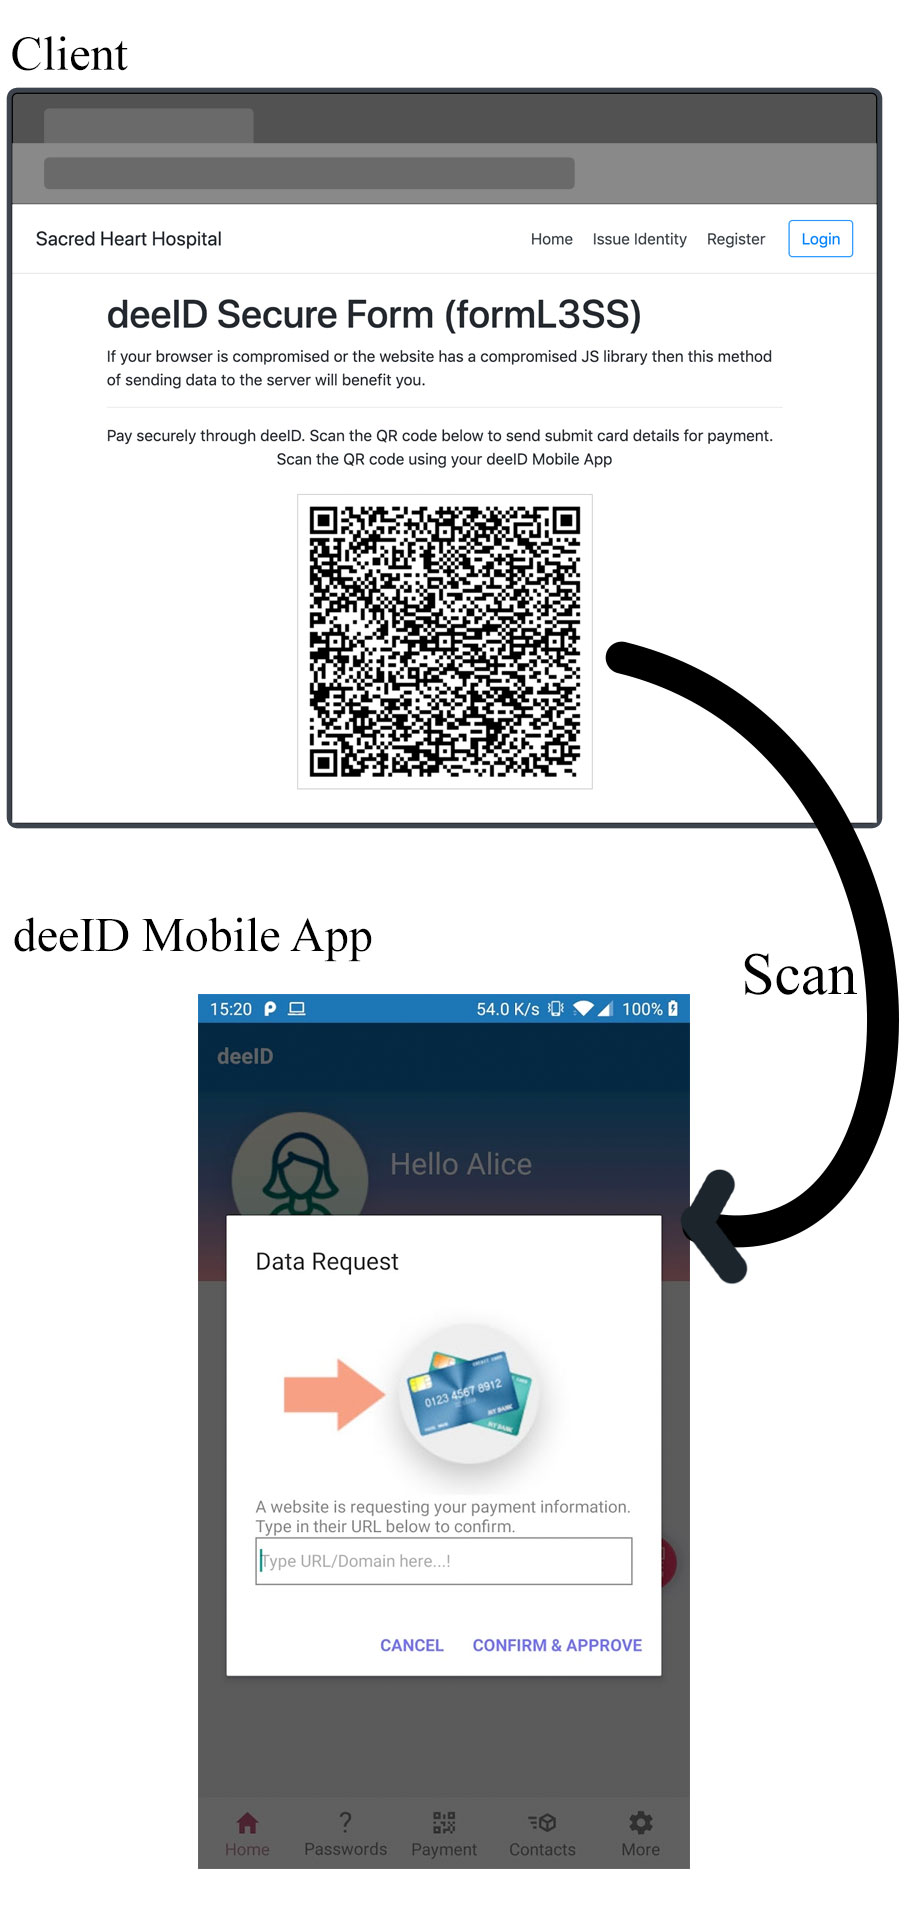
\includegraphics[scale=0.15]{figs/forml3ss/imp.jpg}
\caption{Interface design of the web page and the mobile phone app. Upon scanning the image the mobile app will ensure the QR code's data is not manipulated by verifying the domain and its cryptographic signature.}
\label{fig:imp}
\end{figure}

\paragraph{Backend Functionalities.} The acting server (trusted web server) in our implementation picks up a user journey where the input of a user is required. In our context, we want the user to send a debit or credit card detail to the trusted server. Listing~\ref{lst:backend} shows the data structure sent from the server, it is requesting payment information from the user.

\begin{listing}[H]
\begin{minted}
[
frame=lines,
framesep=2mm,
baselinestretch=0.9,
fontsize=\footnotesize,
]
{python}
qr_msg = json.dumps({
        'type': 'deeIDForm',
        'domain': '',
        'uID': '', #Unique client & WS connection ID
        'form_type': 'card_details',
        'y': y, #Variable to link to a user session
        'exp_time' : '',
        'deeID': deeID, #Websites deeID address
        'sig' : str(sig), #Signature
        'ws_url': ws_url, #WebSocket URL 
    })
\end{minted}
\caption{Data structure and example of data behind the QR code. These data are signed and sent from the trusted server hosting the application the user is interacting with.}
\label{lst:backend}
\end{listing}

\paragraph{Frontend Functionalities.} The frontend functionality is simply a QR code encoder. The client receives the data (signed) from the server and the JavaScript will create a QR image out of that data.

\subsection{Mobile Application Functionalities}
Upon reading the QR code from the compromised computer, the mobile application will attempt to verify the content and its signature. At this point the threat is that malicious actors could have a phishing server setup and have completely changed the content of the QR image to point to the phishing server. We mitigate using the following methods.

\begin{itemize}
    \item If this is our first interaction with the server then we ask the user to type in the domain of the site they have visited; then cross check it with the one in the QR image. The mobile app will then verify the public-key from the server.
    \item If this is not our first interaction with the server then we may verify the identity of the server that signed the QR code with the identity we have associated with the server.
\end{itemize}

Note, phishing threats are minimised through the \deeid ecosystem if we have already established a connection with a service. This relationship is stored and any incoming communication is always verified with the stored information. 

\vspace*{-0.5cm}
\subsection{WebSocket Functionalities}
\vspace*{-0.2cm}
The purpose of the WebSocket server is to create a dynamic and user friendly application; that is to connect the client, server and the mobile phone. It is to allow each device to be updated upon state changes in other devices.


\subsection{Custom Form}
We implemented a simple custom form functionality. This functionality allows the developer to request information that is not in the standardised form requests (currently payment and personal information). In the request data we have a \texttt{custom} \texttt{form\_type}. This also requires another field named \texttt{form}; which is an array of the form fields required. As you can see in the Listing \ref{lst:customform}, we have requested a secret question and answer from the user. This then allows the mobile application to display the right form inputs as seen in Figure \ref{fig:customform}. This figure shows the two form fields requested by the trusted web server.

\begin{listing}[H]
\begin{minted}
[
frame=lines,
framesep=2mm,
baselinestretch=0.9,
fontsize=\footnotesize,
]
{python}
{
    'type': 'deeIDForm',
    'form_type': 'custom',
    'form': [
        ['text', 'Secret question', 'sec_ques_1'],
        ['text', 'Answer', 'sec_ans_1'],
    ],
    ...
}
\end{minted}
\caption{Snippet of the QR code's data when a custom form is implemented. An extra \texttt{form} field to insert an array of required form fields.}
\label{lst:customform}
\end{listing}

\begin{figure}[H]
\centering
\textbf{Custom Form Implementation}\par\medskip
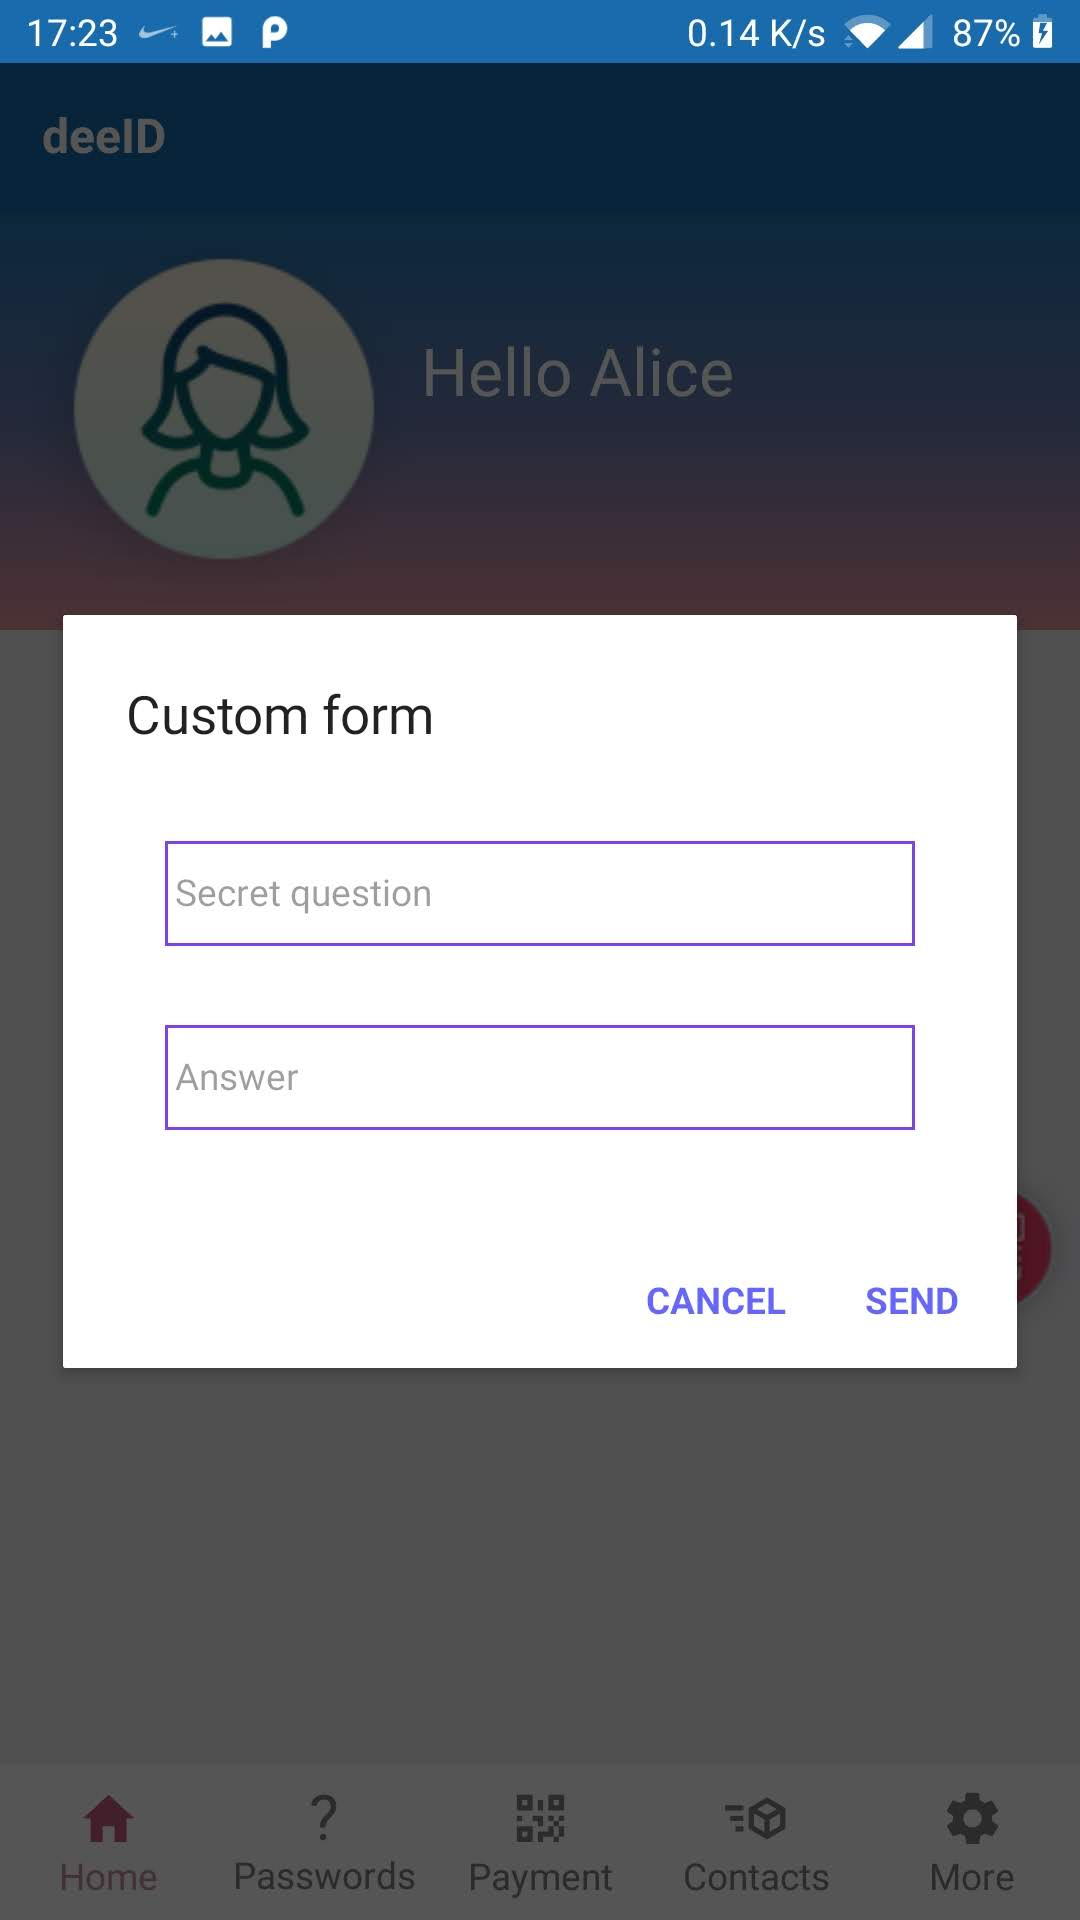
\includegraphics[scale=0.1]{figs/forml3ss/customform.jpg}
\caption{Custom form interface design. Implementation example showing a server requesting two pieces of information.}
\label{fig:customform}
\end{figure}

\section{Alternative Designs}
\label{sec:altdes}
In Section \ref{sec::forml3ss::design} we described a simple design based on the objective of circumventing MitB threats and form grabbers. In this section we will explore different designs and architectures that have different benefits and can be more suited to a given web application. These alternative designs utilise more of the \deeid functionalities: messaging server (being able to send messages to the user's mobile phone without using SMS), encryption and alternative keys stored on the user's \deeid and the \deeid mobile phone app itself.

The following factors determine the suitability of a design:
\begin{itemize}
    \item Complexity of the form: QR code might not be suitable for a complex form.
    \item User and web server relationship: Is the user already registered with the trusted server?
    \item Whether the user has coupled a messaging server with their identity contract.
\end{itemize}

\subsection{User is Registered with the App and has a Messaging Server}
\label{sec::chp6::des1}

If a user is already registered with the website of interest and they have a messaging server associated with their \deeid contract then we can use this method.

\textbf{Remark:} We assume the user is able to use the password-less and out-of-band authentication method with the server.

The server, on request from the client, can send a secure message to the user's mobile phone application via their messaging server requesting a form to be filled in and sent back. Given that the user is already registered with the service they can verify whether it is a phishing threat (cross-checking domain, public-keys used to sign a message, etc.) and its veracity.

\subsection{User is Registered with the App and Has No Messaging Server}
\label{subsec:des2}
Continuing from previous design but assuming there is no messaging server on the user's \deeid contract. The trusted server (hosting the website) can encrypt the QR code data, send it to the client where it can be read by the \deeid mobile phone application and be decrypted. From hereon the process continues as per the first design.

\subsection{Send WebSocket Server and Request Form from Server}
\label{subsec:des3}
If the form (assuming a custom type form) is complex and thus cannot be fully transferred via a QR code; or perhaps the developer is looking for a more dynamic approach to form filling (e.g. the form is split into sections where an answer to one section will determine the type and content of consequent sections) then this method can be used.

Instead of sending all of the form in the QR code, we only send the URL of the trusted WebSocket server (belonging to the website of interest). Upon being verified by the user on their \deeid mobile phone application, the user will begin requesting the form from the WebSocket server. At this point the process is a simple back and forth conversation between the two trusted devices.

\section{Usability Evaluation}

We evaluate the usability of \formless using the framework by Bonneau \etal\ in \textit{The Quest to Replace Passwords}~\cite{bonneau_quest_2012}. We used this method to evaluate \deeid in the previous chapter. We utilise the the usability section of the framework for \formless as well; the deployability and security aspects of the framework are more authentication focussed so they are not used here.

\begin{enumerate}
\item \textbf{Memorywise-Effortless}: \formless is built around \deeid from the previous chapter and therefore stores secrets and sensitive data on the mobile phone device. This eliminates the need to memorise information. Users may need to use a PIN to unlock their device or app, however, this is common operation for most users and with the advent of biometrics it is not a significant usability issue.

\item \textbf{Scalable-for-Users}: \formless can store many sets of data on the mobile phone device. Scalability is not an issue for the user or the system itself.

\item \textbf{Physically-Effortless}: Authentication involves scanning a QR code and confirming submission, a straightforward process comparable to tapping a card, though it assumes consistent carrying of the mobile device.

\item \textbf{Easy-to-Learn}: The interface is simple and familiar; it involves scanning QR codes or following simple instructions on the device.

\item \textbf{Efficient-to-Use}: The process is quick. The network operations would often take few seconds on most LTE or broadband networks. The user does not need additional software on their client, only the mobile app on their mobile phone device.

\item \textbf{Infrequent-Errors}: Most of the functions are deterministic and environmental factors do not impact it. QR code scanning might introduce some source of errors (e.g. if the mobile phone camera is unable to read the QR code), however, with most modern hardware we do not foresee this being an issue.

\item \textbf{Easy-Recovery-from-Loss}: This is a limitation of the current design and implementation. \formless in its current form has no recovery methods.
\end{enumerate}

\section{Discussion}
\label{sec::chp7::discussion}

Our objective has been to circumvent threats from Man-in-the-Browser malware and form grabbers. Specifically, to deny them from exfiltrating use secrets. These types of attack have been around for more than a decade, and they are here to stay. They are becoming much more sophisticated in targeting their victims and evading defences. Targeted attacks against banks and even cryptocurrency exchanges~\cite{moshailov_gozi_2019} using a mix of techniques are becoming more common now. MitB Trojans and form grabbers have primarily targeted web-based payment services and hence are commonly referred to as banking or financial malware. The primary goal of MitB and form grabbers is to essentially steal information that is being typed into a form or turn the user's actions against them (e.g. sending funds to the attacker's bank account if the user is attempting to transfer funds).

It is clear that the threat from MitB and form grabbers is significant. The British Airways case is an example of the scale of the threat. We can defend against these threats through preventive techniques that would guard the user's machine from being infected, and detection techniques that would detect and eliminate the threat. However, our method has been to circumvent the threats, most helpful to a paranoid user. Moreover, whilst it is hard for the prevention and detection techniques to guard against form grabbers, our proposed system can defend the user from such a threat.

The proposed system, \formless, is an out-of-band system that uses a mobile phone device to securely send data to the trusted server that hosts the website.

Prevention and detection techniques have their own benefits. However, an out-of-band system can have superior user experience and security benefits. In the same form, data are always removed from the user experience of a website. With the proposed system that is combined with \deeid the user can store information that is commonly required from websites, such as payment and personal information, on the device (in this case a mobile phone). This stored information can be requested with the proposed standardisation of requests; e.g. payment information is requested by a \texttt{form\_type} being \texttt{card\_info}. Standardising data requests is one of the contributions of this chapter. Targeted information such as payment information can be standardised so that all devices know what data to send in order to satisfy the server without the server explicitly stating the input fields required. This reduces communication overhead.

Given that we have built on top of \deeid, which in itself is a formless and password-less authentication scheme, the system can also defend against phishing attacks. Moreover, \deeid plays an important role, as identification is crucial when dealing with sensitive information online. We consider commonly shared sensitive information to be personal information (name, date of birth, address, etc.) and payment information. These are then interlinked with the identity. Hence, the benefit of using \deeid, an identity system with \formless, is that it can increase security with respect to identity theft and financial fraud. Providing the information and also proving one's identity on the fly adds an extra layer of security.

Malware attacks from banking to ransomware attacks are becoming more sophisticated. Collaboration between criminal gangs~\cite{noauthor_business_2019} and targeted attacks~\cite{cohen_gozi_2019} enables better penetration and quicker responses to the security guards put up by individuals and organisations. IBM predicts~\cite{noauthor_ibm_2019} that using cryptocurrency, criminal gangs are shifting to targeted ransomware attacks because they can evade security forces and launder their money more effectively.

\formless shares conceptual similarities with systems such as Apple Pay and Google Pay. Both make it convenient to carry out a function securely. We can take inspiration from these systems to use NFC for example to transmit data at physical points of \textit{sale}. \formless extends the principle of out-of-band secure transmission to arbitrary web form data using a different technical approach suited to the web browsing context. Using QR codes has become a common method of payment in China using the likes of WeChat---clear evidence that this method of transacting PII or payment can be scalable and reach wide adoption.

The proposed system also has its own limitations. Mobile phones are also susceptible to malware attacks. As the use of mobile phone devices increases, they become more of an attractive target for malicious actors~\cite{szongott_evaluating_2012}. The fact that the user has to use an additional device to submit the form is an additional burden. However, one can argue that because they are so common it is less of a burden. Also, because the user does not constantly type in the same information, the process of submitting sensitive information is easier and more user friendly. The proposed system used \deeid, an experimental technology that generates additional complexities.

\section{Related Work}
\label{sec:rel}
As far as we know, there are no other similar works in which a general form submission protocol is used with a mobile phone and a blockchain PKI system. However, there are similar works with respect to circumventing Man-in-the-Browser and compromised browser threats.

Software-based solutions that circumvent MitB threats include the likes of \fun{TrustJS}~\cite{goltzsche_trustjs:_2017} and \fun{ShadowCrypt}~\cite{he_shadowcrypt:_2014}. \fun{TrustJS} enables trustworthy execution of JavaScript inside a browser by using trusted hardware (Intel SGX in their case) and a browser extension. This enables the validation of the input of the form on the client side. \fun{ShadowCrypt} enables encrypted input/output and runs as a browser extension. Although it is successful in preventing the DOM from containing sensitive data and thus being accessible to other extensions and compromised libraries, it does not prevent keyloggers and other sophisticated Trojans. \fun{Privly}~\cite{noauthor_privly_nodate} performs similar functions to \fun{ShadowCrypt} but also uses a third-party server for encrypted data management.

\fun{Fidelius}~\cite{eskandarian_fidelius_2019} uses additional hardware to completely secure the I/O. In \fun{Fidelius}, the entire I/O path is protected by having a trusted device between the monitor/keyboard and the compromised computer. The drawbacks of \fun{Fidelius} are page load times and display response latency, as additional hardware and operations of the keyboard and display affect the user experience. We think that our proposal enhances the user experience by eliminating the input of data that is already securely stored on the mobile phone. Also, since nothing is required on the browser, there is no impact on page load and response rates. \fun{Bumpy}~\cite{mccune_safe_2009} is similar to \fun{Fidelius} and can be considered a predecessor to \fun{Fidelius}.

\section{Summary}
\label{chp7::sec::summary}
In this chapter, we have discussed the threats from Man-in-the-Browser malware and form grabbers, highlighting the importance of these threats with recent examples. We propose a design to protect the user from compromised browsers and client-side or frontend code.

We have designed an out-of-band solution using a mobile phone named \formless. This system circumvents MitB and form grabbers safely while improving the user's experience whilst interacting with the website. We implemented this design on top of an out-of-band authentication and blockchain-based system, \deeid. We believe that the combination of technologies used is a novel contribution. Moreover, a first in proposing a standard messaging format for out-of-band form submission systems. Developers can request payment and personal information without explicitly defining the form; this reduces communication overhead. Other data can be requested using a \texttt{custom} tag.

Future work include: website identification using \deeid, to add an extra level of security; refining the messaging standard between the trusted server and the user's mobile phone; implementation of the alternative designs that were proposed; and implementing the encryption functions for the transmission of the data.